\section{Final Concept}

The final basic geometry of our final concept is shown in figure \ref{fig:final_concept}. It is important to note that the render does not include all components such as the propellant feed system and propellant diffuser, and that the design may very well look different as we move through the design process. However, it does the job of conveying some of the design goals and choices that have been made. The final concept will consist of the following features:

\begin{enumerate}
    \item Magnetic Field System - will consist of a ferromagnetic core with permanent magnets to create the required magnetic field topology. This will reduce power consumption and avionics system complexity
    \item Cathode - will be centrally mounted on the thruster axis allowing for a more compact design.
    \item Ring anode - simple and well understood design
    \item Propellant feed system - will consist of a pressure vessel, custom propellant diffuser, and supporting hardware. May become to primary conductor to the anode.
\end{enumerate}

As seen in the figure, the addition of a hollow cathode means that the design will revolve around the design of the \ac{AHT}s. Since we are building a thruster that is larger than normal \ac{CHT}s, the downsides of \ac{AHT}s such as wall losses and erosion are not as pronounced. Additionally, the \ac{AHT} architecture is well understood and documented, which will make the design process easier.

As mentioned in section \ref{sec:centrally-mounted-cathode}, can be tedious to integrate into the design of the thruster. Taking this into consideration, it may be advantageous to develop initial prototypes of the thruster with an externally mounted cathode, in that case that the cathode integration is holding up testing. 

\begin{figure}[H]
    \centering
    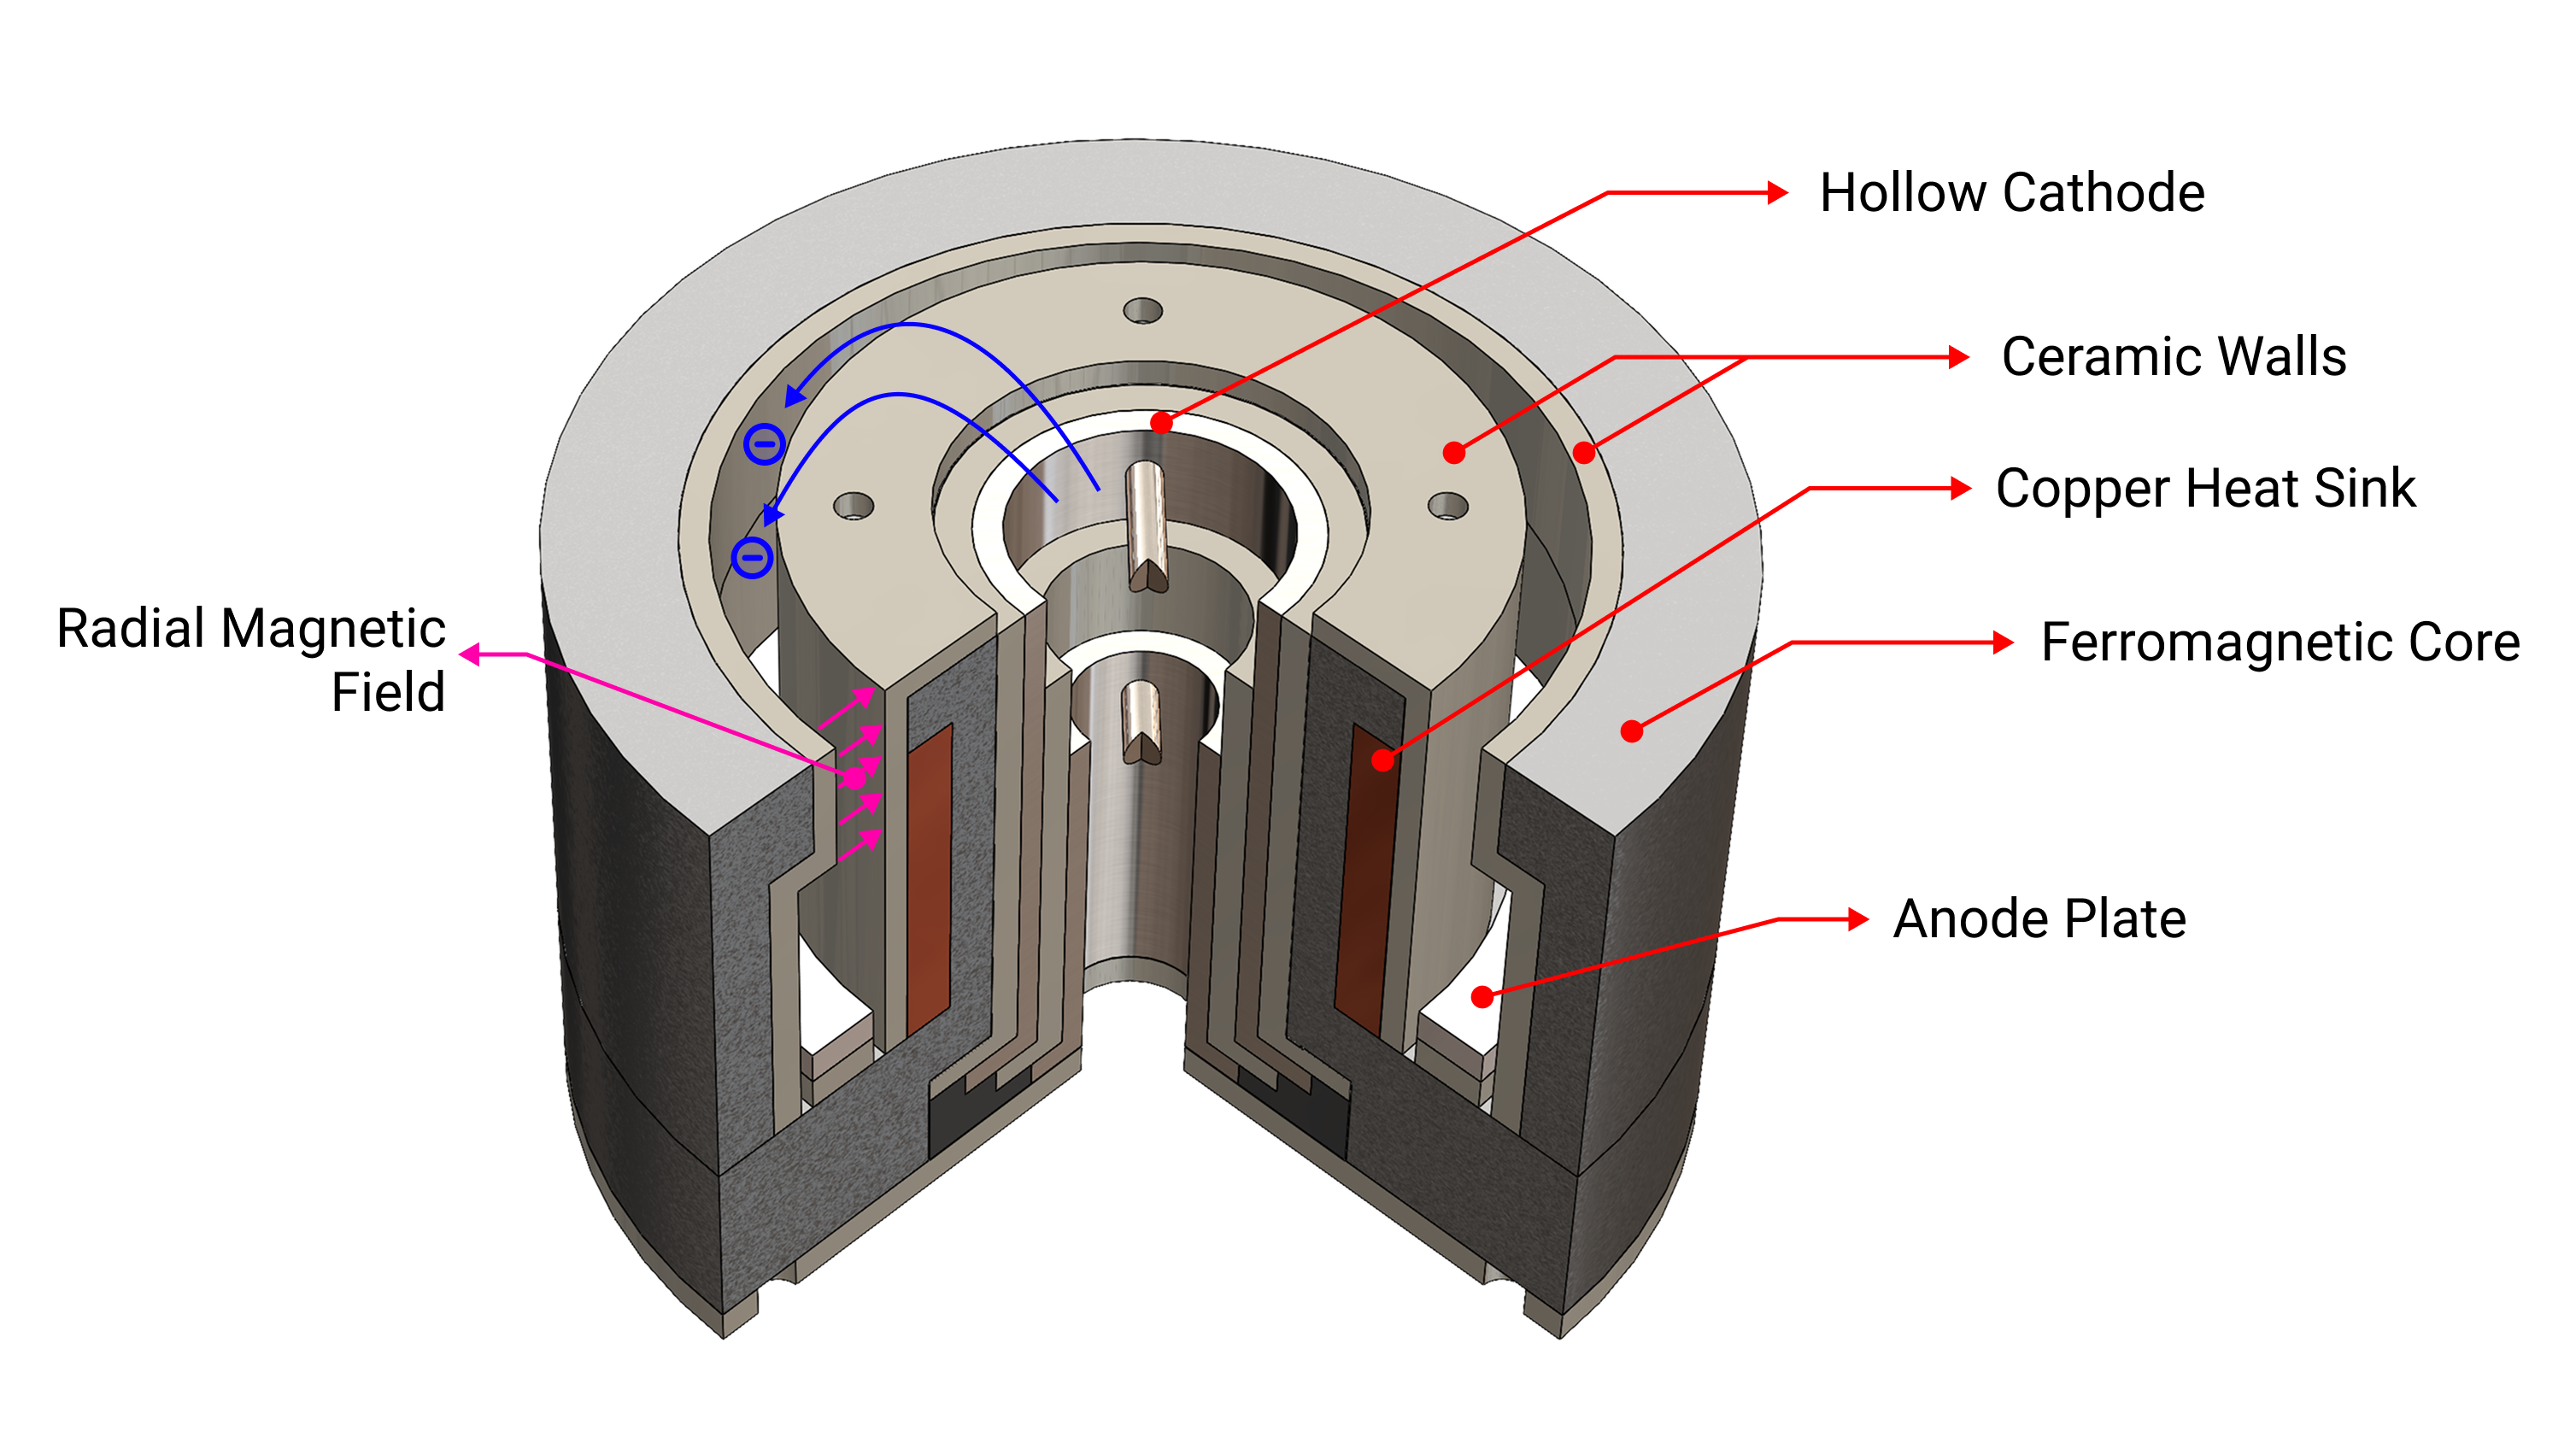
\includegraphics[width=1.0\textwidth]{images/Concepts/final concept.png}
    \captionsetup{justification=centering}
    \caption{Final Concept Diagram}
    \label{fig:final_concept}
\end{figure}